\chapter{Literature Review}
\label{chapter:lit}
This initial literature review supports this project by identifying current practices and characteristics of the frameworks in question, providing foundational metrics to build a virtual project, and synthesize the current understanding of the application of systems engineering frameworks to R\&D and scientific infrastructure projects. 
This is a \textit{non-exhaustive} search and review of publications and research from the last decade. 
It focuses on determining how different frameworks influence project structure, maturity, and performance, particularly in medium-scale research space.\\
The review aims to just begin to answer the following guiding questions:
%%%% Supporting Research Questions %%%%%%%%%%%%%
%\begin{enumerate}
    %\item What qualitative and/or quantitative evidence exists to demonstrate impact of systems engineering as a practice on medium-scale research infrastructure or equivalent projects?
    %\item What are metrics of project success for medium-scale research infrastructure projects?
    %\item What elements of a project are well-understood to impact success metrics?
    %\item What are the characteristics of each framework that map to project elements that impact success?
%\end{enumerate}
%%%%%%%%%%%%%%%%%%%%%%%%%%%%%%%%%%%%%%%%%%%%%%%%
\begin{itemize}[noitemsep, topsep=0pt]
    \item What are the defining characteristics of the OpenSE framework, and how do these compare to minimal and NASA frameworks?
    \item What advantages or limitations have been reported in applying traditional systems engineering frameworks to scientific infrastructure projects?
    \item How has systems engineering been adapted for use in research-oriented scientific collaborations?
    \item How are research infrastructure project measuring their success and which metrics are most transferable to a simulation-based evaluation?
    \item Where do gaps exist in modeling and simulation-based comparisons of framework performance in scientific research contexts?
\end{itemize}
\section{Framework Characteristics}
\label{sect:characteristics}
\subsection{NASA Systems Engineering Framework}
\label{sub:nasa}
The NASA Systems Engineering (SE) framework, formalized in NASA Procedural Requirements (NPR) 7123.1D \cite{npr7123.1D} and detailed in the NASA Systems Engineering Handbook \cite{nasa2016handbook}, defines a structured systems engineering approach that will "enhance NASA's core engineering capabilities while improving safety, mission success, and affordability."\cite{npr7123.1D}. It is a multidisciplinary, lifecycle approach that integrates hardware, software, and human elements at all levels of hierarchy of a system. The framework divides the project lifecycle into Formulation and Implementation phases, each containing well-defined reviews with specified entrance and exit criteria. Each gate verifies that a project is in compliance with NPR 7123.1D and in turn validates its intent to ensure the end product meets the customer's need.\cite{npr7123.1D}

The NASA SE Framework is characterized by Common Technical Processes, Tools and Methods, and Workforce. Figure \ref{fig:nasa_se_framework} illustrates the view that the systems engineering capability increases along the increase of those 3 axes. \\
\begin{figure}[h]
  \centering
  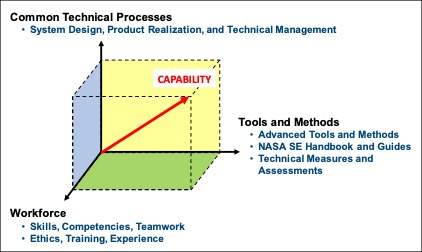
\includegraphics[width=0.7\linewidth]{figures/NPR7123.1DC1F4.jpg}
  \caption{NASA Systems Engineering Framework
  \cite{npr7123.1D}.}
  \label{fig:nasa_se_framework}
\end{figure}

This indicates a deeply embedded systems engineering culture that has explicit roles and job functions of systems engineers to support this framework. 
The framework’s strengths include clear accountability, comprehensive documentation and guidance, and alignment with agency-wide standards. 
The common technical processes mentioned here are defined at the Systems Engineering Engine \cite{npr7123.1D} that are comprise of 17 Technical Processes that are guided by the methods specified in the NASA SE Handbook \cite{nasa2016handbook} and other guiding documents. The 17 Technical Processes are:
\begin{enumerate}[noitemsep, topsep=0pt]
    \item Stakeholder Expectations Definition
    \item Technical Requirements Definition
    \item Logical Decomposition
    \item Design Solution Definition
    \item Product Implementation
    \item Product Integration
    \item Product Verification
    \item Product Validation
    \item Product Transition
    \item Technical Planning
    \item Requirement Management
    \item Interface Management
    \item Technical Risk Management
    \item Configuration Management
    \item Technical Data Management
    \item Technical Assessment
    \item Decision Analysis
\end{enumerate}
\subsection{OpenSE Framework}
\label{sub:opense}
OpenSE was developed within CERN’s Engineering Department as a systems-engineering approach explicitly tailored for scientific facilities \cite{cern2016opense,bonnal2018opense}. 
It was motivated by the recognition that research infrastructures differ fundamentally from aerospace or defense projects: they are collaborative, distributed, constrained by limited documentation cultures and evolving experimental designs, and must balance that with a focus on safety and reliability in the face of facilities with ionizing radiation. 
OpenSE aims to preserve the benefits of structured lifecycle management while reducing unnecessary process overhead.\\
The framework defines six phases (Initialize, Study, Design, Build, Commission, and Finalize) that parallel the ISO/IEC/IEEE 15288 lifecycle but with greater allowance for iteration and concurrency. \\
\begin{figure}[h]
  \centering
  
\includegraphics[width=0.9\linewidth]{figures/openSElifecycle.png}
  \caption{OpenSE Lifecycle
  \cite{cern2016opense}.}
  \label{fig:openSE_lifecycle}
\end{figure}

The framework notes in several places the inspiration from the NASA SE Handbook but that is more specialized and emphasizes tailorability from simple to more advanced approaches to the application of this framework. \cite{cern2016opense}
OpenSE emphasizes four guiding principles: openness, leanness, participation, modularity, and scalability.\cite{cern2016opense}
These principles shift the emphasis of governance that NASA takes through NPR 7123.1D \cite{npr7123.1D} and toward a minimal oversight expect safety kind of approach. The activities OpenSE describes are:
\begin{itemize}[noitemsep, topsep=0pt]
    \item Needs and Requirements 
    \item Integration
    \item Verification and Validation
    \item Solution Finding
    \item Safety Documentation
\end{itemize}
and are adapted from NASA's 17 Common Technical Processes.
\subsection{Minimal Frameworks}
\label{sub:minimal}
In contrast to structured or formal frameworks, many scientific collaborations, especially medium-scale research infrastructure, operate using minimal or ad hoc project management and subsequent systems engineering structures.
These approaches are characterized by limited lifecycle documentation, informal change control, if any, and reliance on experienced team leads for integration oversight rather than formal systems engineering artifacts. 
Most systems engineering practices are not highlighted as practices derived from this discipline but are largely viewed as compliance measure to meet facility requirements but are often considered after large portions of the research infrastructure are fabricated and assembled.
For this reason, there are not technical processes to discuss except derived characteristics which include Principle Investigator (PI)-driven design and facility requirements.
These will be referenced as Solution Finding, Integration, System Safety Verification, and ES\&H Documentation.
\subsection{Comparative Summary}
\label{sub:comparison}
Amongst the 3 approaches, NASA SE represents the most formalized and prescriptive model, emphasizing completeness, documentation, and mission assurance. 
OpenSE, while rooted in the same lifecycle principles, explicitly adapts these practices for research environments, reducing overhead while preserving modularity and openness. 
Minimal frameworks, by contrast, prioritize flexibility and speed at the cost of being formally verifiable and reproducible. 
The comparative characteristics of these frameworks, as synthesized from the literature, are summarized in Table \ref{tab:framework_comparison}.
\begin{table}[h]
\centering
\caption{A Summary of Common Elements Across Frameworks}
\label{tab:framework_comparison}
\begin{tblr}{
  colspec={|X[1.2,l]|X[1.5,l]|X[1.5,l]|X[1.5,l]|},
  hlines,
  row{1} = {font=\bfseries, halign=c},
  column{1} = {font=\bfseries},}
Characteristic & NASA SE & OpenSE & Minimal \\

Lifecycle Structure &
Sequential and gated &
Iterative and facility-driven &
Informal or project-defined \\

Problem Definition &
Stable once defined. 
Significant resources dedicated to requirements development. &
Functional requirements evolve while safety requirements are stable. 
Moderate resources dedicated to requirements development. &
Minimal time spent on requirements development. 
Reactive to safety and facility requirements. \\

Interface Management \& Integration &
Formalized.
Governed by ICDs. &
Structured but more flexible. 
Focuses on collaboration and shared understanding. &
Implicit and unstructured. 
Usually through verbal agreements or minimal documentation, as required by facility. \\

Verification \& Validation &
Formalized, following required V\&V plans. &
Formalized, following required V\&V plans. &
Informal or reactive to facility verification needs. 
Validation relies on in situ testing. \\

Flexibility &
Low to moderate. 
Suited for stable requirements. &
Moderate to high. 
Suited to evolving designs. &
High to very high. 
Suited for rapid development and changes. \\

Type/Domain &
First of a kind and high-stakes/aerospace, defense, missions. &
First or one of a kind, long-term, and iterative/research infrastructures, accelerators. &
First of a kind, demonstrators or prototypes/detectors, instruments, and bench-top R\&D labs. \\

Design \& Solution Finding &
Formalized and driven by agreed-upon requirements. 
Robust, multidisciplinary engineering studies. &
Somewhat formal with robust engineering. 
Driven by needs and requirements. 
Driven by physicists who act as both customer and engineer. &
Informal. 
Driven by PI needs. 
Driven by physicists who act as both customer and engineer. \\

Documentation \& Configuration Management &
Extensive, standardized artifacts. 
Robust engineering controls. &
Lean, scaled to project size. 
Engineering controls. &
Minimal, variable by team. 
Some or little engineering controls. \\
\end{tblr}
\end{table}

The characteristics were selected based on common activities or functions found across each framework.

\section{Advantages and Limitations of Systems Engineering}
\label{sect:pros&cons}

\paragraph{Advantages}
Many studies have been conducted over the last decade or more verifying the benefits of systems engineering. In an effort to not recreate many meta-analyses that already exist, this review will pull from well-known and established resources, primarily the Systems Engineering Book of Knowledge (SEBoK) \cite{sebok_economic_value}. In the review of the economic benefits of systems engineering in SEBoK, a study highlighting the criticality of systems engineering for NASA missions is discuessed. Figure \ref{fig:se_investments} illustrates the relationship between the percentage of project resources devoted to systems engineering and the percentage of project cost overrun.\cite{sebok_economic_value} \\

\begin{figure}[h]
  \centering
  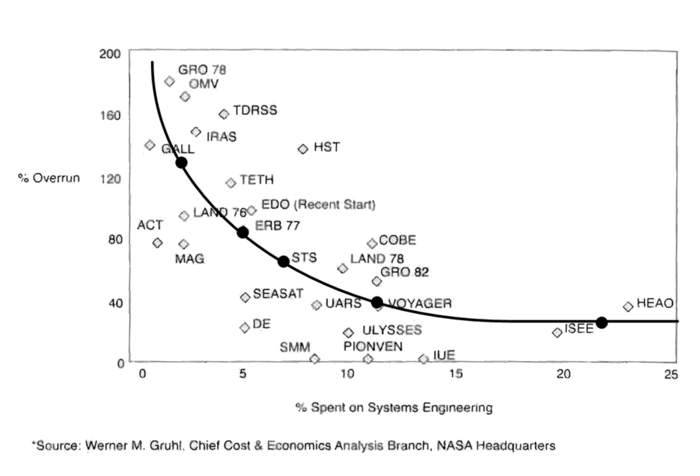
\includegraphics[width=0.7\linewidth]{figures/700px-NASA_Image_Part_1.png}
  \caption{Relation of SE Investments to NASA Program Cost Overruns (Stutzke 2005)
  \cite{sebok_economic_value}.}
  \label{fig:se_investments}
\end{figure}

Data from NASA programs show that projects investing less than 5\% in systems engineering experienced overruns exceeding 150\%, while those allocating greater than 15\% maintained very low overruns. 
This trend demonstrates that robust systems engineering practices reduce technical and programmatic with some enhanced cost and schedule predictability. 
According to this study, even a modest increase in systems engineering investment yields significant benefits in project controls success. 
The gap here is understanding the impacts on this correlation if system performance or mission success were factored in.\\
It is evident that there needs to have a balance struck on time and resources spent on systems engineering and complexity of a system or project.\cite{sebok_economic_value} 
The relationship between the percentage of project time devoted to initial architectural design and risk resolution versus the total schedule impact, including rework, is illustrated in Figure \ref{fig:enoughSE}. 
 
\begin{figure}[h]
  \centering
  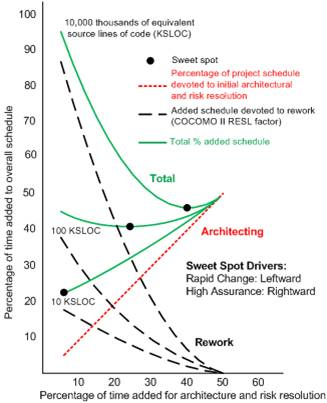
\includegraphics[width=0.7\linewidth]{figures/P1_EconValueSE_RiskBalancedfig2_BB.jpg}
  \caption{Risk-Balanced “How Much SE Is Enough” (Boehm, Valerdi, and Honour 2008)
  \cite{sebok_economic_value}.}
  \label{fig:enoughSE}
\end{figure}

There is clear optimum or "sweet spot" where fairly moderate early investment in architecture and risk management minimizes overall schedule growth. 
Projects that spend too little time in these early phases face substantial rework later, while excessive early analysis can also extend schedules unnecessarily. Physicist and engineers alike can fall prey to "analysis paralysis."
Effective systems engineering finds the balance, ensuring that sufficient effort is applied early to reduce downstream uncertainty and rework, ultimately improving schedule efficiency and project assurance.
Most systems engineering frameworks, if structured well, provide precisely that: tailorability in application (even the more rigid frameworks). 
And that is at the heart of what question being asked here - what is "enough" for medium-scale research infrastructure projects and is OpenSE a viable tailored framework? 
Bonnal et al.\cite{bonnal2018opense} describes OpenSE as “particularly suited to particle-accelerator studies and development projects,” noting its flexibility for projects with shared governance and partial reuse of existing infrastructure (i.e., facility infrastructure from previous experiments).

\paragraph{Limitations}
Multiple analyses have noted that the strengths of rigid systems engineering can impose significant administrative overhead and reduce flexibility when applied to small or exploratory projects \cite{r&dSE}. 
The rigor of NASA SE can thus exceed the practical capacity of medium-scale research infrastructure projects or research-driven teams, particularly those operating with evolving scientific objectives or limited dedicated engineering staff.
Kaeske et al. \cite{Kaeske_Wagner_Albers_Russenschuck_2024} discuss the usefulness of the framework but highlight the needs for more prescriptive methodology and tool support to bridge the gap between intentional generalizations and practical guidance.
Honoré-Livermore et al. \cite{academicsPerceptionSE} and Hodges and Granados \cite{r&dSEbridge} highlight that early-stage R\&D projects often view traditional systems engineering as incompatible with their culture of rapid iteration and discovery. 
Instead, these early-stage R\&D projects apply systems engineering principles selectively, focusing on design and documentation only when required for compliance with a funding organization or the facility hosting the system.

\paragraph{Identified Gaps and Solutions for R\&D}
There is this term called the “Valley of Death” that typically arises at Technology Readiness Levels (TRLs) 5 and 6, where responsibility transitions from early-stage research to full-scale development. 
This phase often becomes a point of friction between exploratory R\&D engineers and those focused on later development at TRLs 7 and higher.\cite{r&dSE} 
Many efforts fail to progress beyond this stage due to insufficient funding, performance gaps, or inadequate mechanisms to bridge research outputs with operational capability. 
Additional causes include unclear research objectives (requirements), poorly managed risks, weak coordination between transitioning organizations (knowledge and interface management), and ineffective application of processes (training and methods). 
Misaligned performance measures, leadership conflicts, and entrenched cultural factors can further exacerbate the issue. 
Ultimately, the findings keep coming back to selecting and implementing the right framework for the project at hand.

\section{Research Infrastructure Project Metrics}
\label{sect:metrics}
So how do we choose the right framework for the project at hand?
The first step might be to characterize what goals the project is trying to achieve and how it intends to measure its success at getting to those goals.
Limited studies or interviews exist to quantify how research experiments, beyond individual experiments of physics runs, quantify success, highlighted by Stotz and Drews.\cite{experimentMetrics} The metrics they did discover after their study were grouped into six categories: 
\begin{enumerate}
    \item \textbf{Volume:} scale and reach of experimentation
    \item \textbf{Outcome-Based:} results and impact of experimentation
    \item \textbf{Quality:} rigor and reliability of experimentation
    \item \textbf{Engagement and Adoption:} how widely experimentation practices are embraced
    \item \textbf{Process Efficiency:} duration from experiment setup to actionable results
    \item \textbf{Strategic Alignment:} impact on broader organizational goals
\end{enumerate}

These categories can easily be mapped back to typical project metrics that give a foundation for the simulation-based study. Volume translates to uptime, outcome-based translates to earned value, quality translates system performance and data integrity, engagement and adoption translates to customer satisfaction, process efficiency translates to schedule, and strategic alignment translates to stakeholder satisfaction.\\
More specific mapping to the simulation will be discussed in the \ref{chapter:methods}.
\section{Gaps in Simulation-Based Research}
\label{sect:simulations}
To date, this project's efforts have not found any studies or research using simulation-based methods to compare systems engineering frameworks impact to performance in the context of scientific research infrastructure projects. 
Further efforts should be made to find alignment between research that exists in similar domains to inform the future work performed.